\documentclass[12pt,a4paper]{ctexart}
\usepackage{amsmath,amssymb,bm,mathtools}
\usepackage{geometry}
\usepackage{graphicx}
\usepackage{booktabs}
\usepackage{float}
\usepackage{caption}
\usepackage{enumitem}
\usepackage{fancyhdr}
\usepackage{algorithm}
\usepackage{algpseudocode}
\geometry{margin=2.5cm}
\graphicspath{{../实验结果/图表/报告实验/}{实验结果/图表/报告实验/}}
\setlength{\parskip}{0.45em}
\setlength{\parindent}{2em}
\linespread{1.12}
\allowdisplaybreaks

\ctexset{
  section/format = \Large\bfseries\centering,
  subsection/format = \large\bfseries
}

\pagestyle{fancy}
\fancyhf{}
\fancyfoot[C]{\thepage}
\renewcommand{\headrulewidth}{0pt}
\renewcommand{\footrulewidth}{0pt}
\fancypagestyle{plain}{%
  \fancyhf{}%
  \fancyfoot[C]{\thepage}%
  \renewcommand{\headrulewidth}{0pt}%
  \renewcommand{\footrulewidth}{0pt}%
}

\title{数值分析与人工智能综合实验报告\\[4pt]
{\Large 基于 Adam 的卷积神经网络训练：\\[2pt]
数值稳定性、超参数敏感性与梯度误差分析}}
\author{}
\date{}

\begin{document}
\maketitle

\begin{abstract}
本实验以 Adam 优化算法训练小型卷积神经网络（CNN）为研究对象，将数值分析中的迭代法稳定性、收敛性、条件数与有限差分误差分析，与人工智能中的图像分类训练过程结合起来。实验包含三部分：其一，在以对角二次型构造的病态优化问题上，验证梯度下降（GD）的步长稳定域、条件数对收敛速度的影响，以及 Adam 的尺度不变性；其二，用中心差商与自动微分对比，分析神经网络梯度计算中的截断误差与舍入误差；其三，在手写数字数据集上，以三个随机种子重复 Adam 与动量 SGD 的对照实验，并系统扫描学习率 $\alpha$、一阶矩系数 $\beta_1$、二阶矩系数 $\beta_2$ 和稳定项 $\epsilon$。结果表明：GD 的稳定域与理论阈值 $0<\alpha<2/L$ 一致；Adam 对目标函数整体缩放近似不变，但并非无条件稳定，学习率过大时会出现剧烈震荡甚至退化为随机猜测；在本实验的小型 CNN 上，$\alpha=10^{-2}$ 的 Adam 取得最佳测试准确率 $0.9840\pm0.0017$，而 $\alpha=5\times10^{-2}$ 与 $\alpha=10^{-1}$ 分别出现高方差和失效；$\beta_1$ 过大、$\beta_2$ 过小均会降低性能，$\epsilon$ 在 FP32 精度下取默认值 $10^{-8}$ 已足够。中心差商的最优步长约为 $5.6\times10^{-5}$，与“截断误差 $O(h^2)$ 与舍入误差 $O(\varepsilon/h)$ 折中”的理论预测相符。
\end{abstract}

\noindent\textbf{关键词：}数值优化；Adam；卷积神经网络；数值稳定性；超参数敏感性；有限差分；自动微分

\section{问题背景}

\subsection{人工智能中的训练问题}
卷积神经网络（CNN）已成为图像分类、目标检测和医学影像分析等任务的核心模型之一。CNN 的训练本质上是一个高维非凸优化问题：给定训练集 $\{(x_i,y_i)\}_{i=1}^N$，网络参数为 $\theta$，经验风险为
\begin{equation}
L(\theta)=\frac{1}{N}\sum_{i=1}^{N}\ell\bigl(f_\theta(x_i),y_i\bigr),
\end{equation}
其中 $\ell$ 为交叉熵损失，$f_\theta$ 为网络输出。训练通过反向传播计算 $\nabla_\theta L$，再由优化算法迭代更新 $\theta$。在实际训练中，学习率过大可能导致损失振荡或发散，学习率过小则收敛缓慢；不同参数的梯度尺度差异很大，统一步长难以同时适配所有坐标。这些现象都可以从数值分析的角度加以解释。

\subsection{数值分析视角}
从数值分析看，训练算法是一个求解非线性方程 $\nabla L(\theta)=0$ 的迭代法。梯度下降可视为梯度流
\begin{equation}
\dot\theta=-\nabla L(\theta)
\end{equation}
的显式 Euler 离散：
\begin{equation}
\theta_{k+1}=\theta_k-\alpha\nabla L(\theta_k).
\end{equation}
因此，步长 $\alpha$ 的选取、迭代矩阵的谱半径、问题的条件数、浮点舍入误差等概念，直接决定了训练是否稳定、收敛多快。Adam（Adaptive Moment Estimation）在 GD 的基础上引入梯度的一阶、二阶指数滑动平均，对每个坐标构造自适应步长，因而在实践中对梯度尺度不敏感，被广泛用于 CNN、Transformer 等模型的训练。

\subsection{研究问题与贡献}
本实验围绕以下问题展开：
\begin{enumerate}[label=(\arabic*),itemsep=0.3em]
\item 在可解析分析的二次型问题上，GD 的步长稳定域是否与理论阈值一致？条件数如何影响收敛速度？Adam 的尺度不变性表现在哪里？
\item 神经网络梯度由自动微分给出，其数值精度如何？中心差商的截断误差与舍入误差如何折中？
\item 在真实 CNN 训练中，Adam 的学习率、$\beta_1$、$\beta_2$、$\epsilon$ 如何影响收敛速度、数值稳定性和泛化性能？它与动量 SGD 有何差异？
\end{enumerate}

本文的贡献在于：用一个可控的二次型实验建立“理论—现象”的对应关系；用有限差分实验定量展示梯度计算中的两类误差；再用三随机种子的 CNN 实验给出超参数敏感性的统计结果。三部分共同构成“数值分析 + 人工智能”的完整实验链条。

\section{核心算法}

\subsection{CNN 与交叉熵损失}
实验采用一个小型 CNN：输入为 $8\times8$ 灰度图像，依次经过
\[
\begin{aligned}
&\text{Conv}(1\to8,3\times3)\to\text{ReLU}\to\text{MaxPool}(2)\\
&\to\text{Conv}(8\to16,3\times3)\to\text{ReLU}\\
&\to\text{Flatten}\to\text{FC}(256\to32)\to\text{ReLU}\to\text{FC}(32\to10).
\end{aligned}
\]
网络输出 $10$ 维 logits，经 softmax 得到类别概率。交叉熵损失为
\begin{equation}
\ell(\hat y,y)=-\log \hat y_y,\qquad
\hat y=\operatorname{softmax}(z),
\end{equation}
其中 $z$ 为 logits，$y$ 为真实类别。反向传播（等价于反向模式自动微分）给出 $\nabla_\theta L$。

\subsection{Adam 优化算法}
设第 $t$ 步的小批量梯度为 $g_t=\nabla_\theta L_t(\theta_{t-1})$。Adam 维护一阶矩估计 $m_t$ 与二阶矩估计 $v_t$：
\begin{align}
m_t &= \beta_1 m_{t-1}+(1-\beta_1)g_t,\\
v_t &= \beta_2 v_{t-1}+(1-\beta_2)g_t^2,
\end{align}
并作偏差校正：
\begin{equation}
\hat m_t=\frac{m_t}{1-\beta_1^t},\qquad
\hat v_t=\frac{v_t}{1-\beta_2^t}.
\end{equation}
参数更新为
\begin{equation}
\theta_t=\theta_{t-1}-\alpha\frac{\hat m_t}{\sqrt{\hat v_t}+\epsilon}.
\label{eq:adam}
\end{equation}
其中 $\alpha$ 为学习率，$\beta_1,\beta_2\in[0,1)$ 控制历史信息的遗忘速度，$\epsilon>0$ 防止分母过小。默认取 $\alpha=10^{-3}$、$\beta_1=0.9$、$\beta_2=0.999$、$\epsilon=10^{-8}$。算法流程见算法~\ref{alg:adam}。

\begin{algorithm}[H]
\caption{Adam 优化算法}
\label{alg:adam}
\begin{algorithmic}[1]
\Require 初始参数 $\theta_0$，学习率 $\alpha$，矩估计系数 $\beta_1,\beta_2$，稳定项 $\epsilon$
\State $m_0\gets 0,\quad v_0\gets 0$
\For{$t=1,2,\ldots,T$}
  \State $g_t\gets \nabla_\theta L_t(\theta_{t-1})$
  \State $m_t\gets \beta_1 m_{t-1}+(1-\beta_1)g_t$
  \State $v_t\gets \beta_2 v_{t-1}+(1-\beta_2)g_t^2$
  \State $\hat m_t\gets m_t/(1-\beta_1^t)$
  \State $\hat v_t\gets v_t/(1-\beta_2^t)$
  \State $\theta_t\gets \theta_{t-1}-\alpha\,\hat m_t/(\sqrt{\hat v_t}+\epsilon)$
\EndFor
\State \Return $\theta_T$
\end{algorithmic}
\end{algorithm}

\subsection{对照算法}
为评价 Adam 的相对表现，实验使用带动量的 SGD 作为对照：
\begin{equation}
u_t=\beta u_{t-1}+g_t,\qquad
\theta_t=\theta_{t-1}-\alpha u_t,
\end{equation}
其中动量系数 $\beta=0.9$，学习率 $\alpha=0.02$。在二次型实验中还使用普通 GD，以便与解析结果对照。

\subsection{中心差商}
设一元函数 $f$ 充分光滑。中心差商
\begin{equation}
D_h f(x)=\frac{f(x+h)-f(x-h)}{2h}
\label{eq:central}
\end{equation}
逼近 $f'(x)$。由 Taylor 展开，
\begin{equation}
f(x+h)-f(x-h)=2hf'(x)+\frac{h^3}{3}f'''(\xi),
\end{equation}
故截断误差为 $O(h^2)$。另一方面，$f(x\pm h)$ 的浮点求值带有相对误差 $\varepsilon$，差商中的舍入误差约为 $O(\varepsilon |f|/h)$。两类误差的折中决定了最优步长，详见第~\ref{sec:fd-theory}~节。

\section{理论分析}

\subsection{梯度流、显式 Euler 与步长稳定域}
考虑二次型
\begin{equation}
L(\theta)=\frac12\theta^T A\theta,\qquad A=A^T\succ0,
\end{equation}
其中 $A$ 的特征值为 $0<\lambda_{\min}=\lambda_1\le\cdots\le\lambda_d=\lambda_{\max}$。GD 迭代为
\begin{equation}
\theta_{k+1}=(I-\alpha A)\theta_k,
\end{equation}
故
\begin{equation}
\theta_k=(I-\alpha A)^k\theta_0.
\end{equation}
迭代收敛当且仅当谱半径
\begin{equation}
\rho(I-\alpha A)=\max_{1\le i\le d}|1-\alpha\lambda_i|<1,
\end{equation}
即
\begin{equation}
0<\alpha<\frac{2}{\lambda_{\max}}=\frac{2}{L}.
\label{eq:stability}
\end{equation}
当 $\alpha$ 接近上界时，对应最大特征值的分量快速衰减，但对应最小特征值的分量衰减很慢；收敛速度由
\begin{equation}
\rho=\max\bigl(|1-\alpha\lambda_{\min}|,\ |1-\alpha\lambda_{\max}|\bigr)
\end{equation}
控制。条件数 $\kappa=\lambda_{\max}/\lambda_{\min}$ 越大，收敛越慢。这解释了病态问题中 GD 的“锯齿”与停滞现象。

\subsection{Adam 的偏差校正与尺度不变性}
假设梯度在短期内近似平稳，即 $\mathbb E[g_t]\approx g$。由 $m_t$ 的展开
\begin{equation}
m_t=(1-\beta_1)\sum_{i=1}^{t}\beta_1^{t-i}g_i
\end{equation}
可得
\begin{equation}
\mathbb E[m_t]=(1-\beta_1^t)g.
\end{equation}
因此 $\hat m_t=m_t/(1-\beta_1^t)$ 是 $g$ 的无偏估计；同理，$\hat v_t$ 是 $\mathbb E[g^2]$ 的无偏估计。偏差校正的作用在训练初期尤其明显：若不做校正，$m_t$ 与 $v_t$ 都偏向零，更新量会被系统性低估。

若梯度整体放大 $c$ 倍（$g\mapsto cg$，$c>0$），则 $m_t\mapsto cm_t$、$v_t\mapsto c^2v_t$，于是
\begin{equation}
\frac{\hat m_t}{\sqrt{\hat v_t}+\epsilon}
\longmapsto
\frac{c\hat m_t}{c\sqrt{\hat v_t}+\epsilon}.
\end{equation}
当 $\epsilon$ 相对于 $c\sqrt{\hat v_t}$ 可忽略时，更新方向与归一化幅度近似不变，这就是 Adam 的尺度不变性。它使 Adam 对损失函数整体缩放、不同参数梯度尺度差异具有较强鲁棒性。但 $\epsilon$ 破坏了严格的尺度不变性：$\epsilon$ 越大，尺度不变性越弱，更新越接近“未归一化”的梯度法。

此外，在 $\beta_1=\beta_2=\beta$ 的特殊情形下，由 Jensen 不等式有 $|\hat m_{t,i}|\le\sqrt{\hat v_{t,i}}$，因此每个坐标的更新量满足
\begin{equation}
|\Delta\theta_{t,i}|\le\alpha.
\end{equation}
一般情况下 $\beta_1\ne\beta_2$，该比值可能略大于 $1$，但 $\epsilon$ 仍为分母提供下界，使单步更新不会因 $v_t$ 过小而爆炸。这是 Adam 数值稳定性的重要来源。

\subsection{非凸情形下的收敛性}
CNN 的损失函数通常非凸，且不满足全局强凸性，因此不能直接套用二次型的收敛结论。对 $L$-光滑且梯度有界的非凸目标，Kingma 与 Ba 证明了：取递减步长 $\alpha_t=\alpha/\sqrt{t}$ 时，Adam 满足
\begin{equation}
\min_{1\le t\le T}\mathbb E\bigl[\|\nabla L(\theta_t)\|^2\bigr]
=\mathcal O\left(\frac{1}{\sqrt T}\right).
\end{equation}
这一结果说明 Adam 在适当步长下可以保证梯度范数趋于零（到一阶稳定点），但它依赖光滑性、梯度有界等假设，且只给出最坏情况下的次线性速率。Reddi 等人进一步指出，原始 Adam 在某些凸问题上可能不收敛，原因是 $\beta_1,\beta_2$ 的相互作用会使有效步长不单调；AMSGrad 通过维护二阶矩的 running maximum 修复了这一问题。因此，Adam 的“经验上很稳”与“理论上无条件收敛”是两回事，实验中的超参数选择仍然重要。

\subsection{数值稳定性分析}
Adam 的更新分母为 $\sqrt{\hat v_t}+\epsilon$。当某个坐标的梯度长期很小，$\hat v_t$ 可能接近零；若没有 $\epsilon$，更新量 $\alpha\hat m_t/\sqrt{\hat v_t}$ 可能非常大。$\epsilon$ 提供了分母下界，保证
\begin{equation}
\left|\frac{\hat m_t}{\sqrt{\hat v_t}+\epsilon}\right|\le \frac{|\hat m_t|}{\epsilon},
\end{equation}
从而避免除零和溢出。但 $\epsilon$ 过大也会带来偏差：它相当于把自适应更新“拉回”到普通梯度更新，降低有效步长。在 FP32 下，机器精度约为 $1.19\times10^{-7}$，默认 $\epsilon=10^{-8}$ 与 $\sqrt{\hat v_t}$ 的量级相比通常很小；而在 FP16 或混合精度训练中，$\epsilon$ 需要相应放大，否则 $\hat v_t$ 的下溢会使分母失去意义。

学习率 $\alpha$ 是最关键的稳定性参数。由式~\eqref{eq:adam}，$\alpha$ 直接控制全局步长；过大的 $\alpha$ 会使参数在极小值附近来回跳动，损失震荡甚至发散。$\beta_1$ 控制一阶矩的记忆长度：$\beta_1$ 越大，方向越平滑，但对梯度方向变化的响应越滞后；$\beta_2$ 控制二阶矩的记忆长度：$\beta_2$ 越大，自适应分母越平滑，但面对非平稳梯度时可能“过期”，导致步长失配。实际训练中应监控梯度范数、损失曲线和参数更新范数，以便及早发现数值异常。

\subsection{有限差分的截断误差与舍入误差}
\label{sec:fd-theory}
对式~\eqref{eq:central}，由 Taylor 展开，
\begin{equation}
D_hf(x)=f'(x)+\frac{h^2}{6}f'''(\xi)+O(h^4),
\end{equation}
故截断误差约为 $\frac{h^2}{6}|f'''(\xi)|$。另一方面，计算 $f(x\pm h)$ 时的相对舍入误差为 $\varepsilon$，绝对误差约为 $\varepsilon|f|$；两个相近的数相减会损失有效数字，差商的舍入误差约为
\begin{equation}
\frac{\varepsilon|f|}{2h}.
\end{equation}
因此总误差可建模为
\begin{equation}
E(h)\approx C h^2+\frac{\varepsilon|f|}{2h}.
\end{equation}
令 $E'(h)=0$ 得
\begin{equation}
h^*\approx\left(\frac{\varepsilon|f|}{4C}\right)^{1/3}.
\end{equation}
对双精度 $\varepsilon\approx2.2\times10^{-16}$，若 $C$ 与 $|f|$ 同量级，则 $h^*$ 约为 $10^{-5}$ 量级。这预测了误差—步长曲线呈“U 形”：$h$ 太大时截断误差占主导，$h$ 太小时舍入误差占主导。第~\ref{sec:gradcheck}~节的实验将验证这一预测。

\subsection{超参数作用与实验假设}
综合以上分析，提出如下实验假设：
\begin{enumerate}[label=H\arabic*.,itemsep=0.3em]
\item 学习率 $\alpha$ 存在一个稳定上界；超过该上界后，训练损失出现震荡或发散。
\item $\beta_1$ 过大（接近 $1$）会因动量滞后而减慢收敛；$\beta_1$ 适中时收敛较快。
\item $\beta_2$ 过小会使自适应分母对当前梯度过于敏感，导致训练不稳定或性能下降；$\beta_2$ 接近 $1$ 时更平滑，但过大可能对非平稳梯度响应不足。
\item $\epsilon$ 在 FP32 下取默认值附近时影响较小；明显增大 $\epsilon$ 会降低有效步长，减慢收敛。
\item Adam 对目标函数整体缩放近似不变；GD 则不具此性质，步长需随曲率缩放。
\end{enumerate}

\section{编程实践}

\subsection{实验环境}
实验在 Windows 11 上完成，使用 conda 环境 \texttt{jup}：
\begin{itemize}[itemsep=0.2em]
\item Python 3.11；
\item PyTorch 2.14.1（CPU 版）；
\item NumPy 2.4.4、pandas 3.0.2、Matplotlib 3.10.8、scikit-learn 1.7.1。
\end{itemize}
所有随机种子固定，数据划分、模型初始化和小批量顺序均可复现。完整实验脚本为 \texttt{代码/报告实验脚本.py}，图表与数据表分别保存在 \texttt{实验结果/图表/报告实验/} 和 \texttt{实验结果/数据表/报告实验/} 目录。

\subsection{数据与模型}
使用 scikit-learn 自带的 Digits 数据集：共 1797 张 $8\times8$ 灰度手写数字图像，10 个类别。像素值除以 16 归一化到 $[0,1]$。按分层抽样划分为训练集、验证集、测试集，比例为 $70\%/15\%/15\%$，对应 1257/270/270 个样本。

CNN 结构如第~2.1~节所述，参数总量为
\[
80+1168+8224+330=9802.
\]
训练使用交叉熵损失、批量大小 64、18 个 epoch，不使用权重衰减、Dropout 或数据增强，以突出优化算法本身的影响。

\subsection{实验设计}
实验分为三部分。

\textbf{(1) 二次型实验。}取 $d=20$，$A=\operatorname{diag}(\lambda_1,\ldots,\lambda_d)$，特征值在对数尺度上从 $1$ 到 $100$ 均匀分布，条件数 $\kappa=100$。初始点 $\theta_0=(1,\ldots,1)^T$，迭代 1000 步。比较 GD 在 $\alpha=10^{-3},10^{-2},1.9\times10^{-2},2.1\times10^{-2},5\times10^{-2}$ 下的表现；比较 GD、动量法与 Adam 的收敛速度；并考察目标函数放大 $10^3$ 倍时 Adam 与 GD 的差异。

\textbf{(2) 梯度有限差分检验。}在双精度下取一个小批量，用自动微分计算第一层卷积权重的梯度，再对梯度绝对值最大的 8 个坐标用中心差商式~\eqref{eq:central} 计算近似值。步长 $h$ 取 $10^{-8}$ 到 $1$ 之间的 33 个对数等距点，记录相对误差的中位数。

\textbf{(3) CNN 训练实验。}固定数据划分，使用 3 个随机种子（2026、2027、2028）重复每个配置；对每个种子，模型初始化和小批量顺序相同，从而保证不同超参数配置之间的对照是受控的。共扫描 12 个配置：
\begin{itemize}[itemsep=0.2em]
\item 基线：动量 SGD（$\alpha=0.02$，动量 $0.9$）与默认 Adam；
\item 学习率：$\alpha=10^{-4},10^{-3},10^{-2},5\times10^{-2},10^{-1}$；
\item 一阶矩：$\beta_1=0.5,0.9,0.99$；
\item 二阶矩：$\beta_2=0.9,0.999,0.9999$；
\item 稳定项：$\epsilon=10^{-8},10^{-5},10^{-3}$。
\end{itemize}
每个 epoch 记录训练损失、验证损失、验证准确率和平均梯度范数；训练结束后在测试集上计算测试损失与准确率。所有指标报告三个种子的均值与标准差。

\subsection{评价指标与可复现性}
主要指标为测试准确率与测试损失，辅助指标为最终验证准确率和最终平均梯度范数。梯度范数定义为
\begin{equation}
\|\nabla_\theta L\|_2=\Bigl(\sum_{j}\|\nabla_{\theta_j}L\|_2^2\Bigr)^{1/2},
\end{equation}
在每个小批量更新前计算，再对一个 epoch 内的批次取平均。该指标用于观察梯度爆炸、梯度消失以及不同优化器的更新尺度。为保证可复现性，脚本在每次训练前调用 \texttt{set\_seed(seed)}，并为训练数据加载器使用固定种子的 \texttt{torch.Generator}。

\section{数值结果}

\subsection{二次型实验：步长稳定域与尺度不变性}
二次型实验的结果如图~\ref{fig:quadratic}~和表~\ref{tab:quadratic}~所示。理论稳定域为 $0<\alpha<2/\lambda_{\max}=0.02$。实验中 $\alpha=1.9\times10^{-2}$ 稳定收敛，而 $\alpha=2.1\times10^{-2}$ 与 $\alpha=5\times10^{-2}$ 均发散，与理论阈值一致。$\alpha=10^{-3}$ 虽然稳定，但 1000 步后 $f/f_0$ 仍约为 $7.59\times10^{-4}$，收敛很慢；$\alpha=10^{-2}$ 与 $1.9\times10^{-2}$ 分别在 391 步和 206 步内达到 $10^{-6}$。这说明步长不能一味取小：在稳定域内适当增大 $\alpha$ 可以显著加速收敛。

\begin{figure}[H]
\centering
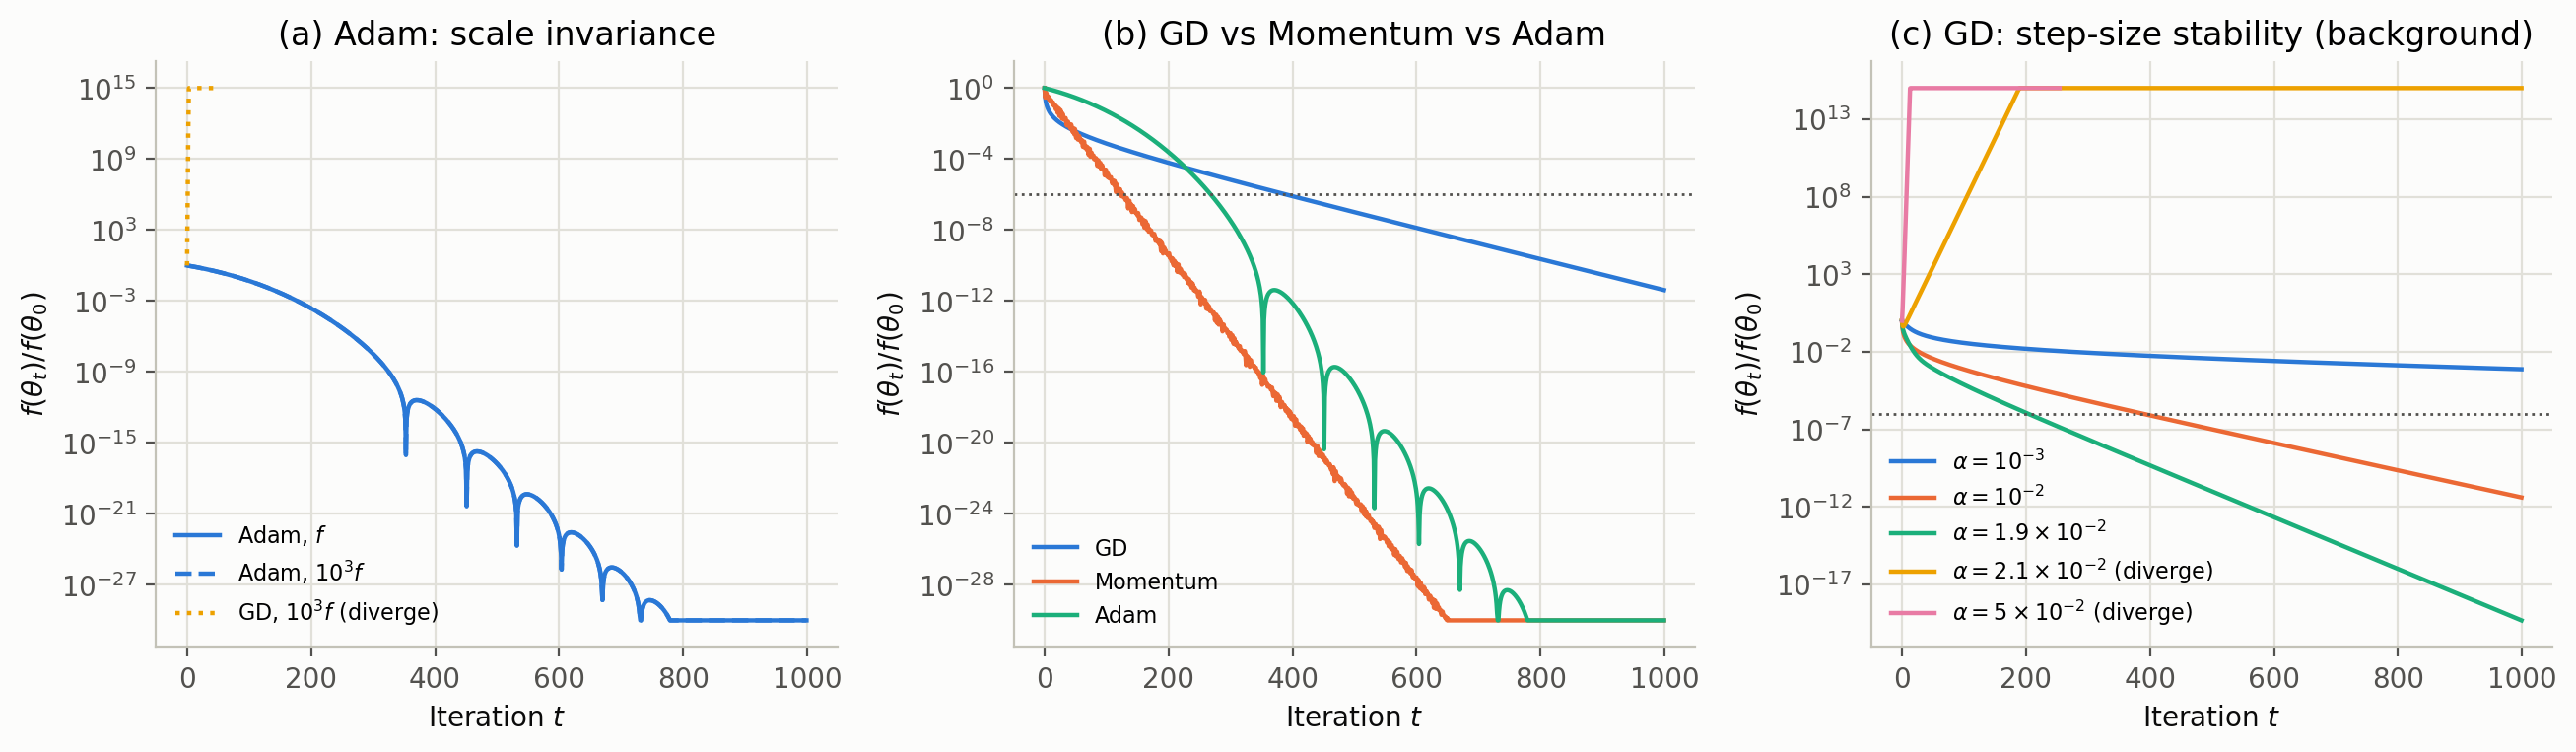
\includegraphics[width=\textwidth]{二次型收敛性与稳定性.png}
\caption{二次型优化实验。(a) GD 在不同步长下的收敛/发散行为，虚线为 $10^{-6}$ 容差；(b) GD、动量法与 Adam 的对比；(c) Adam 的尺度不变性：目标函数放大 $10^3$ 倍后 Adam 的收敛曲线几乎不变，而 GD 发散。}
\label{fig:quadratic}
\end{figure}

\begin{table}[H]
\centering
\caption{二次型实验的收敛表现（$d=20$，$\kappa=100$，1000 次迭代）}
\label{tab:quadratic}
\small
\begin{tabular}{llccc}
\toprule
方法 & 设置 & 是否发散 & 达到 $10^{-6}$ 的迭代数 & 最终 $f/f_0$\\
\midrule
GD & $\alpha=10^{-3}$ & 否 & --- & $7.59\times10^{-4}$\\
GD & $\alpha=10^{-2}$ & 否 & 391 & $4.15\times10^{-12}$\\
GD & $\alpha=1.9\times10^{-2}$ & 否 & 206 & $4.91\times10^{-20}$\\
GD & $\alpha=2.1\times10^{-2}$ & 是 & --- & $1.09\times10^{82}$\\
GD & $\alpha=5\times10^{-2}$ & 是 & --- & $\infty$\\
Momentum & $\alpha=10^{-2},\ \beta=0.9$ & 否 & 125 & $9.05\times10^{-47}$\\
Adam & $\alpha=10^{-2}$ & 否 & 270 & $7.00\times10^{-43}$\\
\bottomrule
\end{tabular}
\end{table}

图~\ref{fig:quadratic}(b) 显示，动量法在 125 步内达到 $10^{-6}$，是三种方法中最快的；Adam 用 270 步，略慢于动量法，但在初期下降很快，随后出现明显的非单调振荡。这一现象与 Adam 的自适应归一化有关：在病态二次型上，不同坐标的有效步长被拉平，最小特征值方向上的更新相对过大，因而产生过冲。它提醒我们，Adam 的“快速初期下降”并不等于“单调收敛”。

图~\ref{fig:quadratic}(c) 验证了尺度不变性：将目标函数放大 $10^3$ 倍后，Adam 的 $f/f_0$ 曲线与原始问题几乎重合；而 GD 在同样的 $\alpha=10^{-2}$ 下发散，因为有效曲率放大了 $10^3$ 倍，违反了稳定域条件。这是 Adam 在实际深度学习中受欢迎的重要原因之一。

\subsection{梯度有限差分检验}
\label{sec:gradcheck}
梯度检验结果如图~\ref{fig:gradcheck}~所示。误差—步长曲线呈明显的 U 形：当 $h=10^{-8}$ 时，中位数相对误差约为 $2.48\times10^{-6}$，舍入误差占主导；随着 $h$ 增大，误差迅速下降，在 $h\approx5.6\times10^{-5}$ 处达到最小值 $3.75\times10^{-10}$；此后截断误差占主导，$h=1$ 时相对误差约为 $0.542$。最优步长的量级与第~\ref{sec:fd-theory}~节的理论预测 $h^*\sim10^{-5}$ 一致。

\begin{figure}[H]
\centering
\includegraphics[width=0.68\textwidth]{梯度有限差分误差.png}
\caption{中心差商与自动微分的相对误差随步长 $h$ 的变化。红色虚线标出中位数误差最小的步长 $h\approx5.6\times10^{-5}$。}
\label{fig:gradcheck}
\end{figure}

该实验有两点意义。第一，它验证了 PyTorch 自动微分实现的正确性：在合适的步长下，中心差商与自动微分的相对误差可达 $10^{-10}$ 量级。第二，它直观展示了数值微分中“截断误差—舍入误差”的经典折中：步长并非越小越好，过小的 $h$ 会因浮点相减损失有效数字而使误差反弹。这一结论对深度学习中的梯度检查、有限差分灵敏度分析等实践具有直接指导意义。

\subsection{CNN 基线对比：Adam 与动量 SGD}
图~\ref{fig:baseline}~给出 Adam 与动量 SGD 在三个种子上的均值曲线，表~\ref{tab:cnn}~给出全部配置的测试指标。基线结果如下：
\begin{itemize}[itemsep=0.2em]
\item 动量 SGD：测试损失 $0.1130\pm0.0135$，测试准确率 $0.9630\pm0.0060$；
\item 默认 Adam：测试损失 $0.1762\pm0.0129$，测试准确率 $0.9481\pm0.0030$。
\end{itemize}
Adam 在前 5 个 epoch 的验证损失下降更快、验证准确率上升更快，体现了自适应步长的初期加速作用；但在 18 个 epoch 结束时，动量 SGD 的验证损失和测试损失都更低，最终测试准确率也略高。图~\ref{fig:baseline}(c) 显示，SGD 的梯度范数在训练中期出现峰值后持续下降，而 Adam 的梯度范数保持在较高水平（约 $1.7$），说明 Adam 的归一化更新并未让梯度本身变小，而是改变了参数更新的尺度。

\begin{figure}[H]
\centering
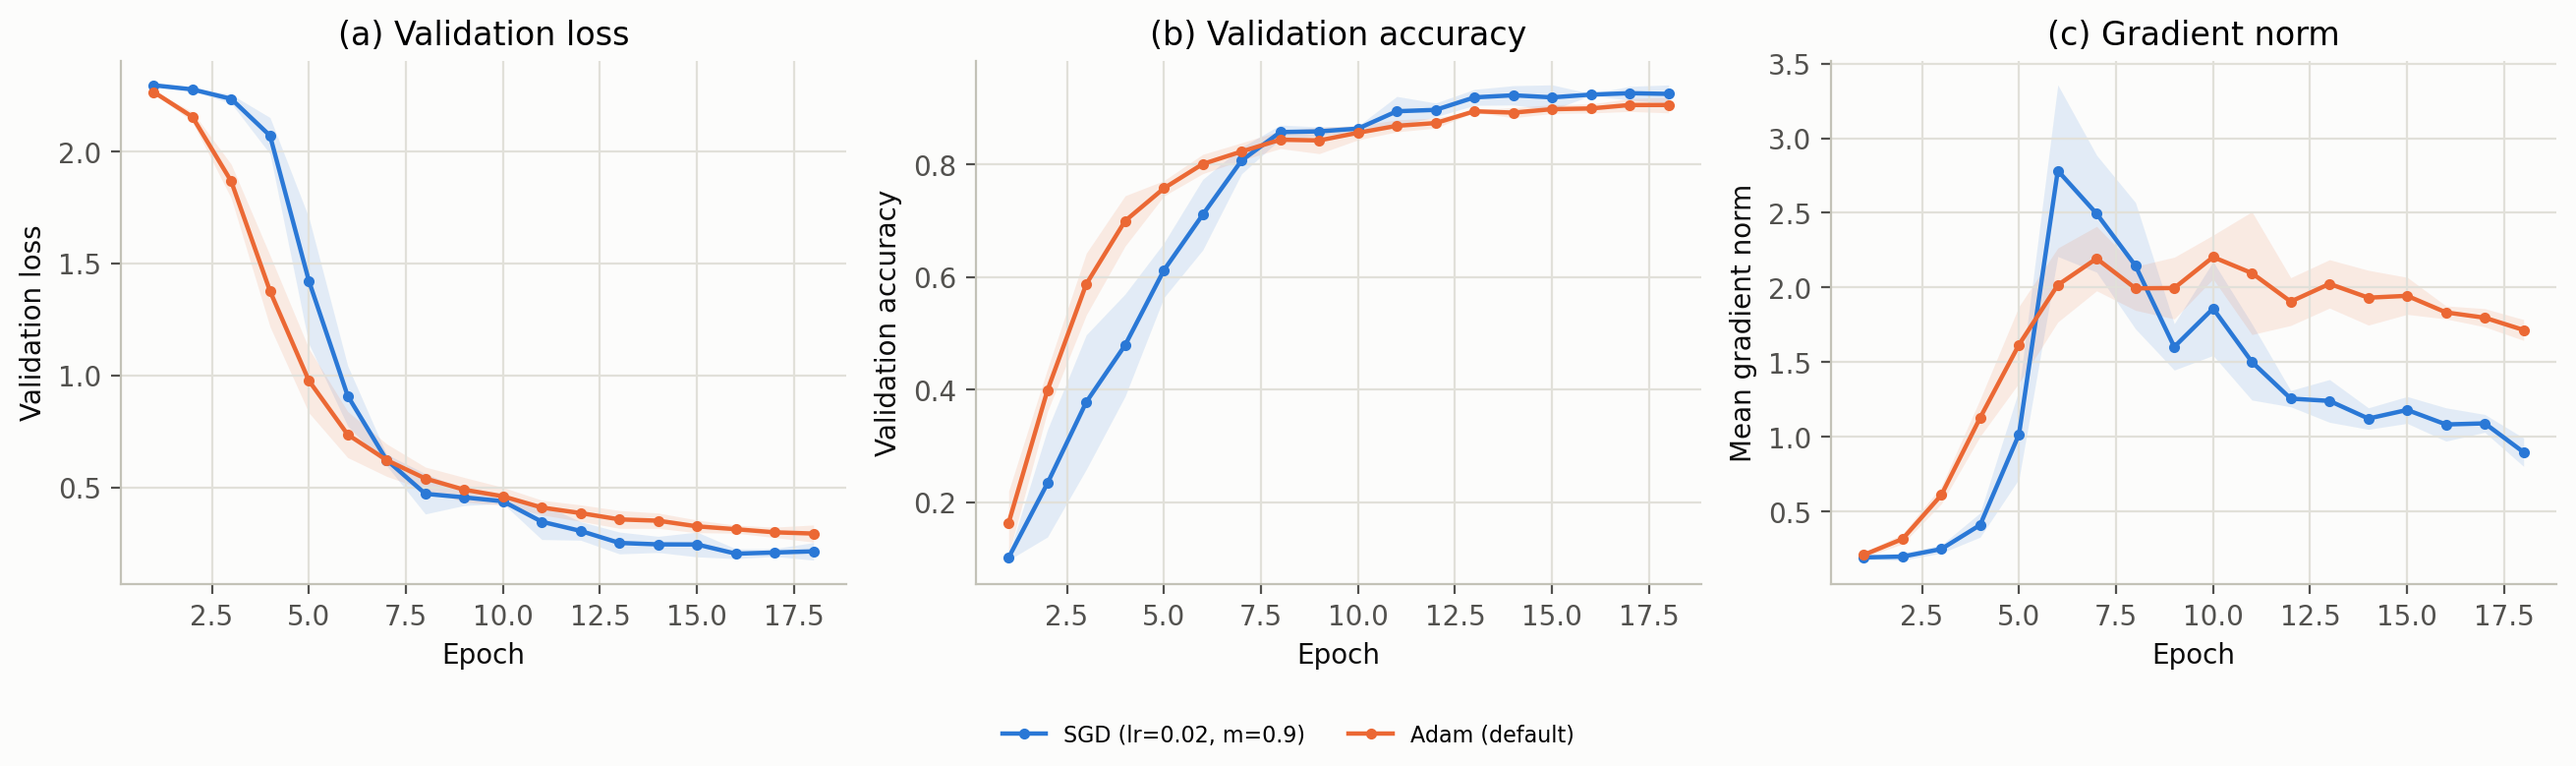
\includegraphics[width=\textwidth]{Adam与SGD基线对比.png}
\caption{Adam 与动量 SGD 的基线对比（三个种子的均值，阴影为标准差）。(a) 验证损失；(b) 验证准确率；(c) 平均梯度范数。}
\label{fig:baseline}
\end{figure}

\subsection{超参数敏感性}

\subsubsection{学习率 $\alpha$}
学习率扫描结果如图~\ref{fig:lr}~所示。$\alpha=10^{-4}$ 时训练几乎停滞，18 个 epoch 后测试准确率仅为 $0.5691\pm0.0501$；$\alpha=10^{-3}$（默认）恢复到 $0.9481\pm0.0030$；$\alpha=10^{-2}$ 取得最佳测试准确率 $0.9840\pm0.0017$，且曲线最平滑。继续增大到 $\alpha=5\times10^{-2}$ 时，三个种子的结果出现巨大分化：测试准确率均值 $0.6642$、标准差 $0.3990$，其中一个种子退化为随机猜测（$0.10$）；$\alpha=10^{-1}$ 时三个种子全部停留在 $0.10$ 左右，训练完全失效。这与第~3.4~节的分析一致：学习率超过稳定范围后，参数更新在极小值附近剧烈震荡，甚至把网络推入 ReLU 大面积失活的退化区域。

\begin{figure}[H]
\centering
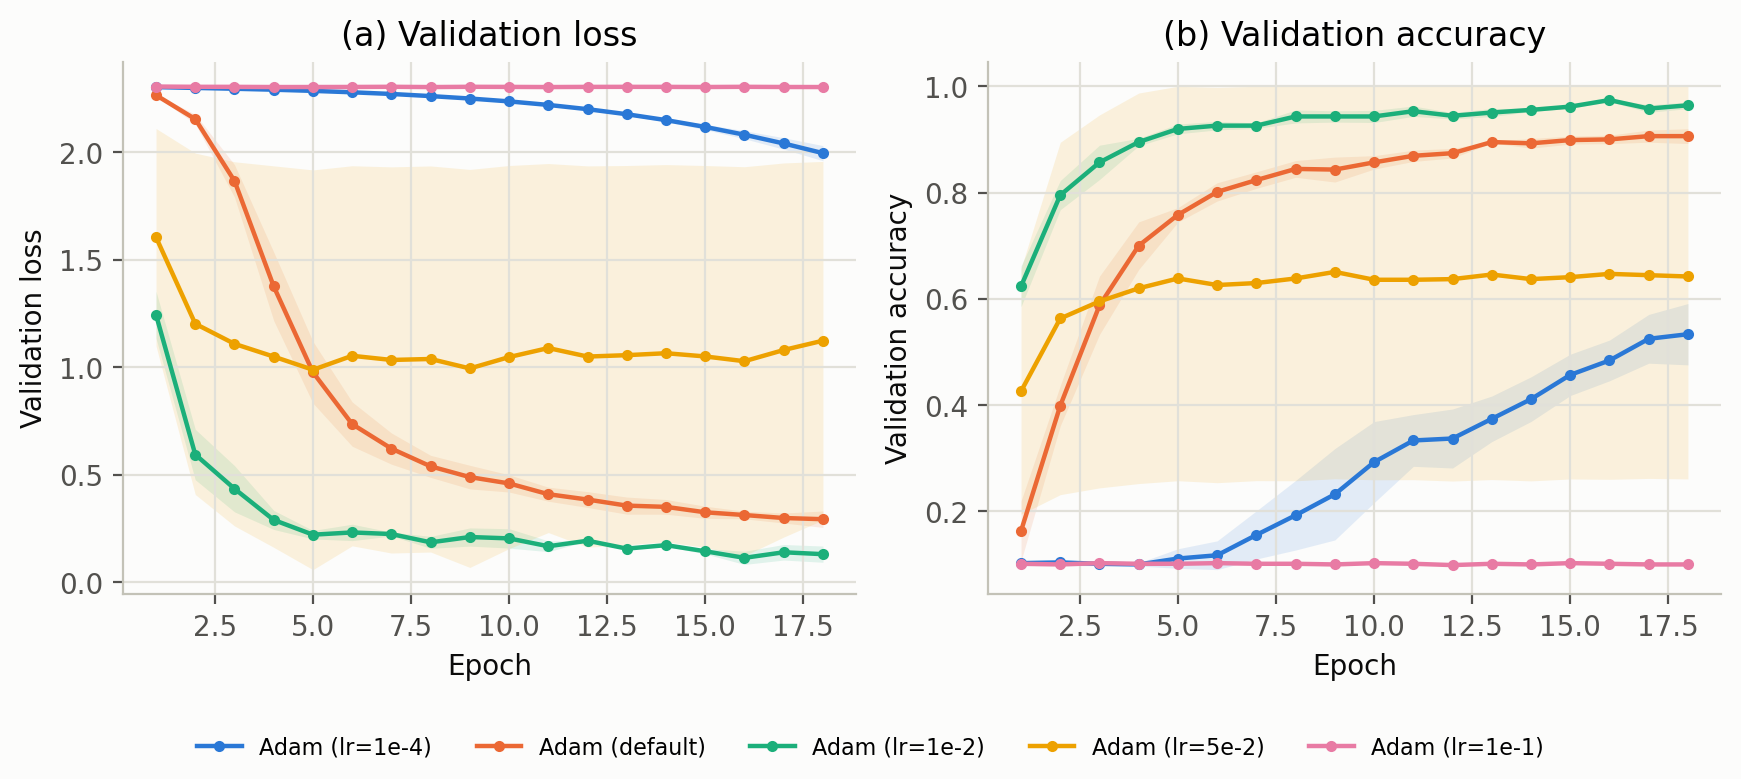
\includegraphics[width=\textwidth]{学习率敏感性.png}
\caption{学习率对 Adam 训练的影响（三个种子的均值与标准差）。(a) 验证损失；(b) 验证准确率。$\alpha=10^{-2}$ 收敛最快且最稳定；$\alpha=5\times10^{-2}$ 出现高方差，$\alpha=10^{-1}$ 失效。}
\label{fig:lr}
\end{figure}

\subsubsection{一阶矩系数 $\beta_1$ 与二阶矩系数 $\beta_2$}
图~\ref{fig:beta}~给出 $\beta_1$ 与 $\beta_2$ 的扫描结果。$\beta_1=0.5$ 时验证损失下降最快，最终测试准确率 $0.9494\pm0.0076$，与默认值 $0.9481\pm0.0030$ 接近；$\beta_1=0.99$ 时动量记忆过长，验证损失下降明显变慢，最终测试准确率降至 $0.9136\pm0.0167$。这说明 $\beta_1$ 过大时，历史梯度方向会滞后于当前损失面的变化，导致收敛变慢。

$\beta_2=0.9$ 时测试准确率降至 $0.9235\pm0.0076$，验证损失也明显高于默认值；$\beta_2=0.9999$ 时测试准确率 $0.9469\pm0.0017$，与默认值 $0.999$ 接近。$\beta_2$ 过小意味着二阶矩对当前梯度过于敏感，自适应分母波动大，等效步长不稳定；$\beta_2$ 过大则对非平稳梯度的响应变慢，但在本实验的短训练中影响不显著。

\begin{figure}[H]
\centering
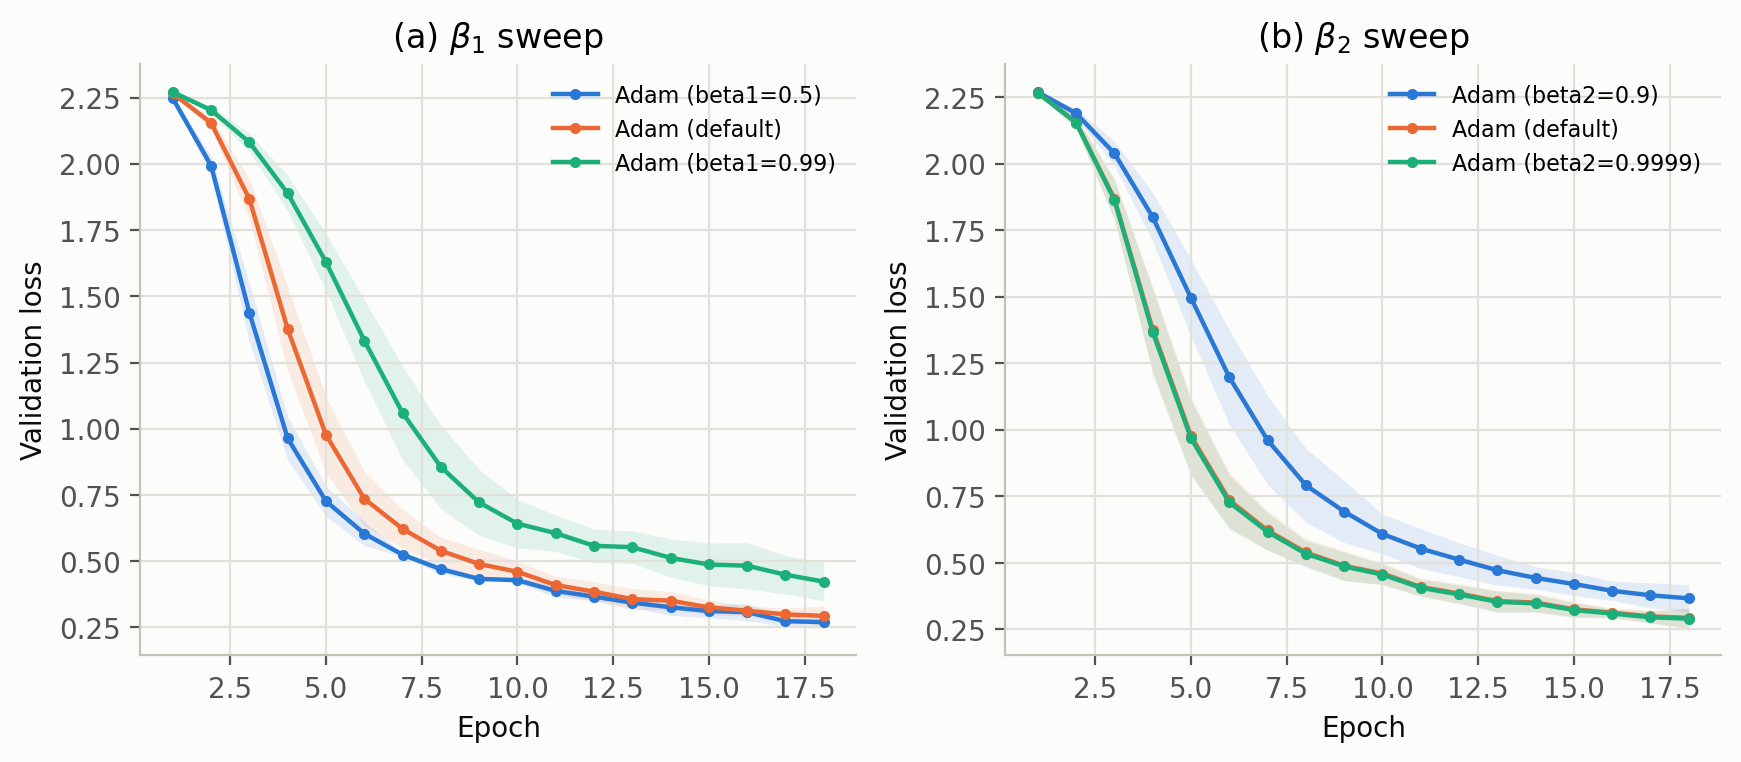
\includegraphics[width=\textwidth]{矩估计系数敏感性.png}
\caption{矩估计系数的影响（验证损失，三个种子的均值与标准差）。(a) $\beta_1$ 扫描：$\beta_1=0.99$ 明显减慢收敛；(b) $\beta_2$ 扫描：$\beta_2=0.9$ 性能下降，$\beta_2=0.9999$ 与默认值接近。}
\label{fig:beta}
\end{figure}

\subsubsection{稳定项 $\epsilon$}
图~\ref{fig:epsilon}~显示，$\epsilon=10^{-5}$ 的曲线与默认 $\epsilon=10^{-8}$ 几乎重合，最终测试准确率 $0.9469\pm0.0035$，差异在统计误差范围内；$\epsilon=10^{-3}$ 则使验证损失下降变慢，最终测试准确率降至 $0.9333\pm0.0080$。这与第~3.4~节的分析一致：在 FP32 下，默认 $\epsilon$ 相对于 $\sqrt{\hat v_t}$ 很小，增大 $\epsilon$ 会削弱自适应归一化的效果，使有效步长变小。需要注意的是，在 FP16 或低精度训练中，$\epsilon$ 的选择会更加关键。

\begin{figure}[H]
\centering
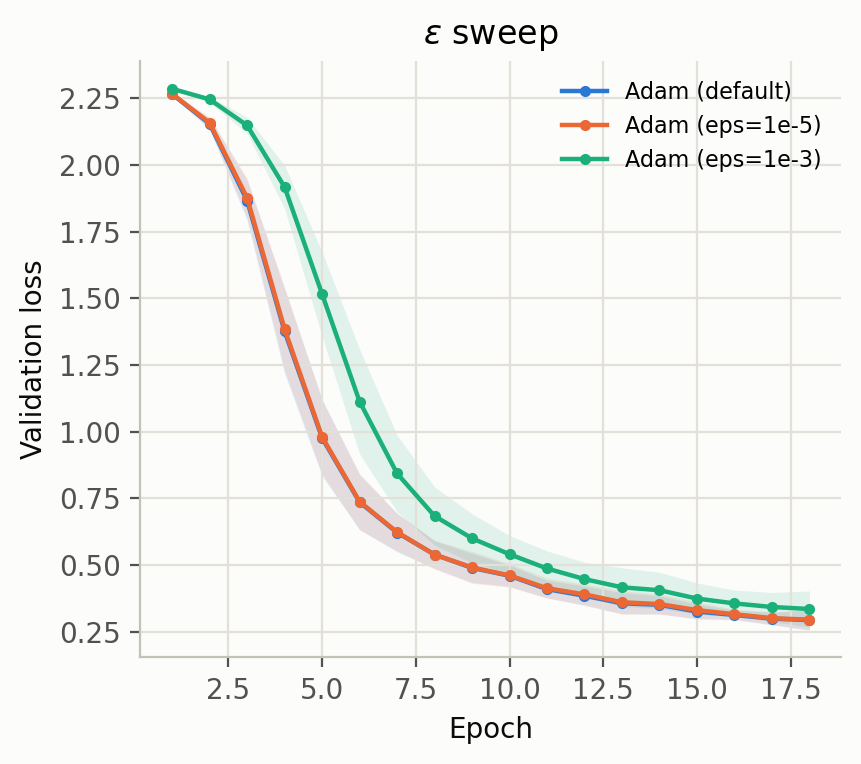
\includegraphics[width=0.72\textwidth]{稳定项敏感性.png}
\caption{稳定项 $\epsilon$ 对验证损失的影响（三个种子的均值与标准差）。$\epsilon=10^{-3}$ 明显减慢收敛；$\epsilon=10^{-5}$ 与默认值几乎一致。}
\label{fig:epsilon}
\end{figure}

\begin{table}[H]
\centering
\caption{CNN 训练实验汇总（三个种子的均值 $\pm$ 标准差；测试集 270 个样本）}
\label{tab:cnn}
\footnotesize
\setlength{\tabcolsep}{4pt}
\begin{tabular}{lcccc}
\toprule
配置 & 测试损失 & 测试准确率 & 最终验证准确率 & 最终梯度范数\\
\midrule
SGD ($\alpha=0.02$, $m=0.9$) & $0.1130\pm0.0135$ & $0.9630\pm0.0060$ & $0.9259\pm0.0160$ & $0.8980\pm0.0951$\\
Adam（默认） & $0.1762\pm0.0129$ & $0.9481\pm0.0030$ & $0.9062\pm0.0140$ & $1.7160\pm0.0696$\\
Adam ($\alpha=10^{-4}$) & $1.9768\pm0.0385$ & $0.5691\pm0.0501$ & $0.5333\pm0.0577$ & $0.6594\pm0.0589$\\
Adam ($\alpha=10^{-2}$) & $0.0537\pm0.0182$ & $0.9840\pm0.0017$ & $0.9642\pm0.0063$ & $0.2235\pm0.0842$\\
Adam ($\alpha=5\times10^{-2}$) & $0.9527\pm0.9569$ & $0.6642\pm0.3990$ & $0.6420\pm0.3810$ & $0.6396\pm0.3697$\\
Adam ($\alpha=10^{-1}$) & $2.3035\pm0.0006$ & $0.1025\pm0.0017$ & $0.1000\pm0.0000$ & $0.1272\pm0.0047$\\
Adam ($\beta_1=0.5$) & $0.1661\pm0.0208$ & $0.9494\pm0.0076$ & $0.9099\pm0.0143$ & $1.6552\pm0.0517$\\
Adam ($\beta_1=0.99$) & $0.2400\pm0.0291$ & $0.9136\pm0.0167$ & $0.8827\pm0.0076$ & $2.8074\pm0.2395$\\
Adam ($\beta_2=0.9$) & $0.2402\pm0.0089$ & $0.9235\pm0.0076$ & $0.8877\pm0.0092$ & $2.1408\pm0.1425$\\
Adam ($\beta_2=0.9999$) & $0.1739\pm0.0135$ & $0.9469\pm0.0017$ & $0.9074\pm0.0157$ & $1.7016\pm0.0708$\\
Adam ($\epsilon=10^{-5}$) & $0.1788\pm0.0133$ & $0.9469\pm0.0035$ & $0.9086\pm0.0126$ & $1.7213\pm0.0531$\\
Adam ($\epsilon=10^{-3}$) & $0.2136\pm0.0125$ & $0.9333\pm0.0080$ & $0.8963\pm0.0157$ & $1.8511\pm0.1460$\\
\bottomrule
\end{tabular}
\end{table}

\subsection{讨论}
综合三部分实验，可以得到以下认识。

\textbf{(1) 稳定性首先由步长决定。}二次型实验给出了清晰的稳定域 $0<\alpha<2/\lambda_{\max}$，CNN 实验则显示 $\alpha=5\times10^{-2}$ 已接近失稳边界、$\alpha=10^{-1}$ 完全失效。尽管 CNN 的损失面非凸、无法直接套用二次型的阈值，但“存在稳定上界、过大步长导致震荡或退化”的定性结论仍然成立。

\textbf{(2) Adam 的自适应性是双刃剑。}尺度不变性使 Adam 对梯度整体缩放和不同坐标的尺度差异不敏感，因而在初期收敛快、调参相对容易；但自适应归一化会拉平不同方向的曲率，在病态问题上造成过冲和非单调行为（图~\ref{fig:quadratic}(b)）。在本实验中，默认 Adam 的最终测试准确率略低于动量 SGD，而 $\alpha=10^{-2}$ 的 Adam 又明显优于两者，说明 Adam 的性能高度依赖学习率，不能简单地说“Adam 一定优于 SGD”。

\textbf{(3) $\beta_1,\beta_2$ 主要影响收敛速度与稳定性。}$\beta_1$ 过大导致动量滞后，$\beta_2$ 过小导致自适应分母波动；这与理论分析一致。默认值 $(0.9,0.999)$ 在本实验的短训练中表现稳健。

\textbf{(4) $\epsilon$ 在 FP32 下不是主要矛盾。}$\epsilon=10^{-8}$ 与 $10^{-5}$ 的差异很小，而 $10^{-3}$ 会明显降低有效步长。这个结论依赖于精度和梯度尺度，不能无条件推广到混合精度训练。

\textbf{(5) 数值分析提供了可检验的解释。}二次型的谱分析、Adam 的偏差校正与尺度不变性、有限差分的截断—舍入折中，都能定量预测实验现象。这种“理论—可控实验—真实任务”的链条，比单纯调参更能说明算法为什么有效、在什么条件下失效。

\textbf{局限性。}本实验使用较小的 Digits 数据集、单一 CNN 结构和 18 个 epoch，训练规模有限；每个配置只有 3 个随机种子，统计波动仍然存在；未使用权重衰减、Dropout、数据增强或学习率调度，因此结论主要反映优化算法本身，而非完整的深度学习工程实践。此外，Adam 的收敛性定理依赖光滑性和梯度有界等假设，CNN 的实际训练并不严格满足这些条件，理论结果应作为定性指导而非严格保证。

\section{结论}
本实验将数值分析与人工智能结合起来，围绕 Adam 训练 CNN 的稳定性与超参数敏感性完成了三组实验。主要结论如下：
\begin{enumerate}[label=(\arabic*),itemsep=0.3em]
\item 二次型实验验证了 GD 的步长稳定域 $0<\alpha<2/\lambda_{\max}$；条件数 $\kappa=100$ 使最小特征值方向收敛缓慢；动量法和 Adam 都能加速病态问题，但 Adam 可能出现非单调过冲。
\item Adam 对目标函数整体缩放近似不变：目标放大 $10^3$ 倍后其收敛曲线几乎不变，而 GD 在相同步长下发散。$\epsilon$ 破坏严格尺度不变性，并在分母上提供数值保护。
\item 中心差商的误差随步长呈 U 形，最优步长约 $5.6\times10^{-5}$，最小相对误差 $3.75\times10^{-10}$，与截断误差 $O(h^2)$、舍入误差 $O(\varepsilon/h)$ 的折中分析一致。
\item 在 Digits 小型 CNN 上，$\alpha=10^{-2}$ 的 Adam 取得最佳测试准确率 $0.9840\pm0.0017$；默认 Adam 为 $0.9481\pm0.0030$，略低于动量 SGD 的 $0.9630\pm0.0060$；$\alpha=5\times10^{-2}$ 出现高方差，$\alpha=10^{-1}$ 失效。
\item $\beta_1=0.99$、$\beta_2=0.9$ 均降低性能；$\beta_1=0.5$ 与默认值接近；$\epsilon=10^{-3}$ 减慢收敛，$\epsilon=10^{-5}$ 与默认值差异很小。
\end{enumerate}
这些结果说明：Adam 的实用性来自动量平滑与自适应归一化的结合，但其稳定性仍受学习率、矩估计系数和数值精度制约；数值分析中的谱分析、误差分析和稳定性理论，可以为深度学习优化器的选择与调参提供可检验的依据。

\begin{thebibliography}{99}
\small
\bibitem{kingma2015}
D.~P. Kingma and J.~Ba.
\newblock Adam: A method for stochastic optimization.
\newblock In \emph{International Conference on Learning Representations (ICLR)}, 2015.

\bibitem{reddi2018}
S.~J. Reddi, S.~Kale, and S.~Kumar.
\newblock On the convergence of Adam and beyond.
\newblock In \emph{International Conference on Learning Representations (ICLR)}, 2018.

\bibitem{goodfellow2016}
I.~Goodfellow, Y.~Bengio, and A.~Courville.
\newblock \emph{Deep Learning}.
\newblock MIT Press, 2016.

\bibitem{nocedal2006}
J.~Nocedal and S.~J. Wright.
\newblock \emph{Numerical Optimization}, 2nd edition.
\newblock Springer, 2006.

\bibitem{burden2016}
R.~L. Burden and J.~D. Faires.
\newblock \emph{Numerical Analysis}, 10th edition.
\newblock Cengage Learning, 2016.

\bibitem{ruder2016}
S.~Ruder.
\newblock An overview of gradient descent optimization algorithms.
\newblock \emph{arXiv preprint arXiv:1609.04747}, 2016.

\bibitem{paszke2019}
A.~Paszke, S.~Gross, F.~Massa, et al.
\newblock PyTorch: An imperative style, high-performance deep learning library.
\newblock In \emph{Advances in Neural Information Processing Systems (NeurIPS)}, 2019.

\bibitem{lecun1998}
Y.~LeCun, L.~Bottou, Y.~Bengio, and P.~Haffner.
\newblock Gradient-based learning applied to document recognition.
\newblock \emph{Proceedings of the IEEE}, 86(11):2278--2324, 1998.
\end{thebibliography}

\end{document}
